\documentclass[10pt,aspectratio=43]{beamer}

\usepackage{graphicx}
\usepackage{tikz}
\usepackage{xcolor}
\usepackage{caption}
\usepackage{subcaption}
\usepackage{bm}
\usetikzlibrary{calc} 
\usepackage{hyperref}
\hypersetup{
    colorlinks=true,
    linkcolor=blue,
    urlcolor=red
}
\usepackage{fontawesome5}
\usepackage{ulem}
\usepackage[dvipsnames]{xcolor}

\usetheme{MyStyle}   % loads beamerthemeMyStyle.sty
\setlength{\columnsep}{0pt}

\usepackage{listings} % for code rendering
\definecolor{codegreen}{rgb}{0,0.5,0}
\definecolor{codegray}{rgb}{0.5,0.5,0.5}
\definecolor{codeblue}{rgb}{0,0,0.7}
\definecolor{codebg}{rgb}{0.96,0.96,0.96}

\lstset{
    language=C++,
    basicstyle=\ttfamily\scriptsize,
    keywordstyle=\color{codeblue}\bfseries,
    commentstyle=\color{codegreen}\itshape,
    stringstyle=\color{red!70!black},
    numberstyle=\tiny\color{codegray},
    backgroundcolor=\color{codebg},
    numbers=left,
    numbersep=6pt,
    frame=single,
    rulecolor=\color{codegray},
    breaklines=true,
    showstringspaces=false,
    tabsize=4,
    columns=fullflexible,
    keepspaces=true,
    morekeywords={nullptr,constexpr,override,final,auto,std,size_t,uint8_t,uint16_t,uint32_t,int64_t}
}


%%%%%%%%%%%%%%%%%%%%%%%%%%%%%%%%%%%%%%%%%%
%%%%%%%%%%%%%%%%%%%%%%%%%%%%%%%%%%%%%%%%%%
%%%%%%%%%%%%%%%%%%%%%%%%%%%%%%%%%%%%%%%%%%

\title{Recap : waveform classification, decoding, hit selection}
\newcommand{\eventname}{AHDC calibration meeting}
\author{Felix Touchte Codjo}
\institute{IJCLab}
\date{November 4, 2026}


\begin{document}

\begin{frame}[plain] % remove header, footer, barre de navigation
\titlepage
\end{frame}

%\begin{frame}{Outline}
%\tableofcontents
%\end{frame}

%\section{Intro}
\section{Updates}


\begin{frame}{Waveform classification}
    \begin{itemize}
        \item The signals recorded by the AHDC have various shapes
        \item These different waveforms need specific treatments
        \item We gather them into seven categories
    \end{itemize}

    \centering
    \vspace{0.15cm}
    {
        \footnotesize
        \begin{tabular}{lll}
            wfType 6 $\rightarrow$ too short & 
                wfType 3 $\rightarrow$ pileup (ongoing work) & 
                    wfType 0 $\rightarrow$ normal \\
            wfType 5 $\rightarrow$ decreasing & 
                wfType 2 $\rightarrow$ missing trailing edge & 
                     \\
            wfType 4 $\rightarrow$ small ToT & 
                wfType 1 $\rightarrow$ saturated & 
                     \\
        \end{tabular}
    }

    \vspace{0.3cm}
    {
        \setlength{\tabcolsep}{1pt}
        \begin{tabular}{cccc}
            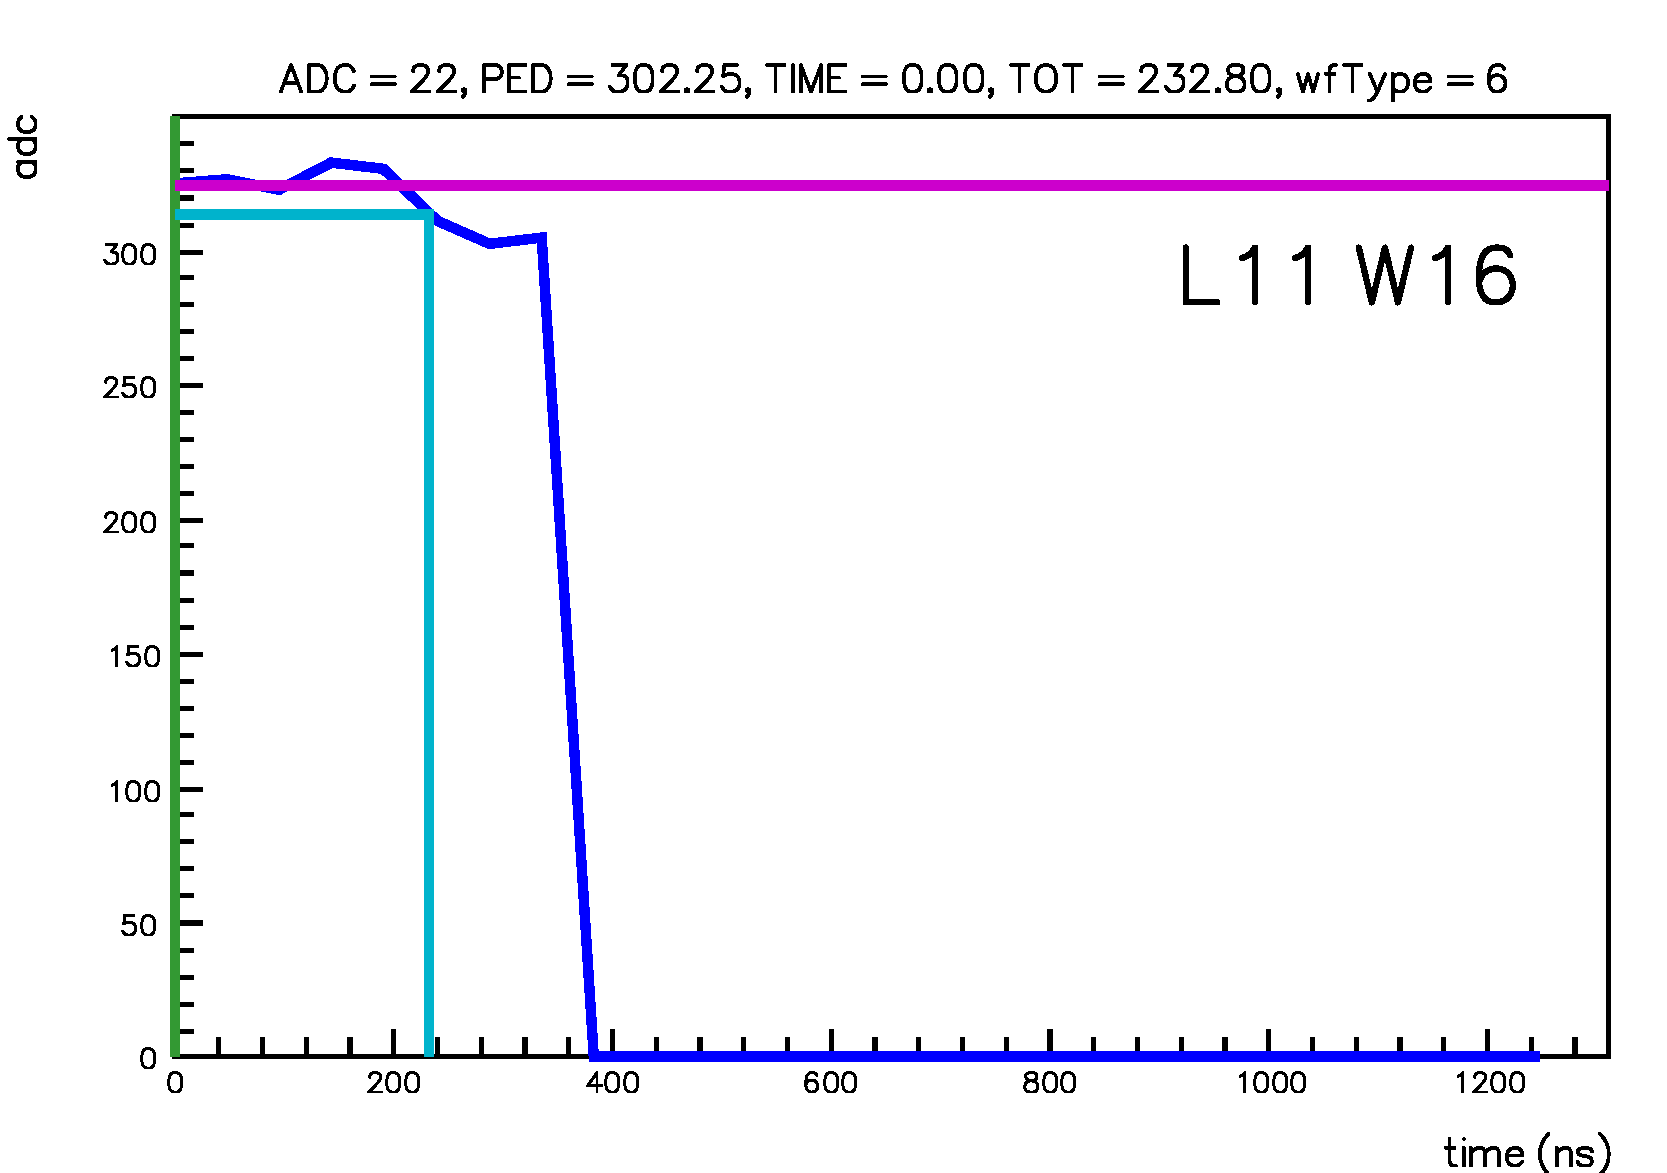
\includegraphics[width=0.24\linewidth]{figures/wf6_short.pdf} &
                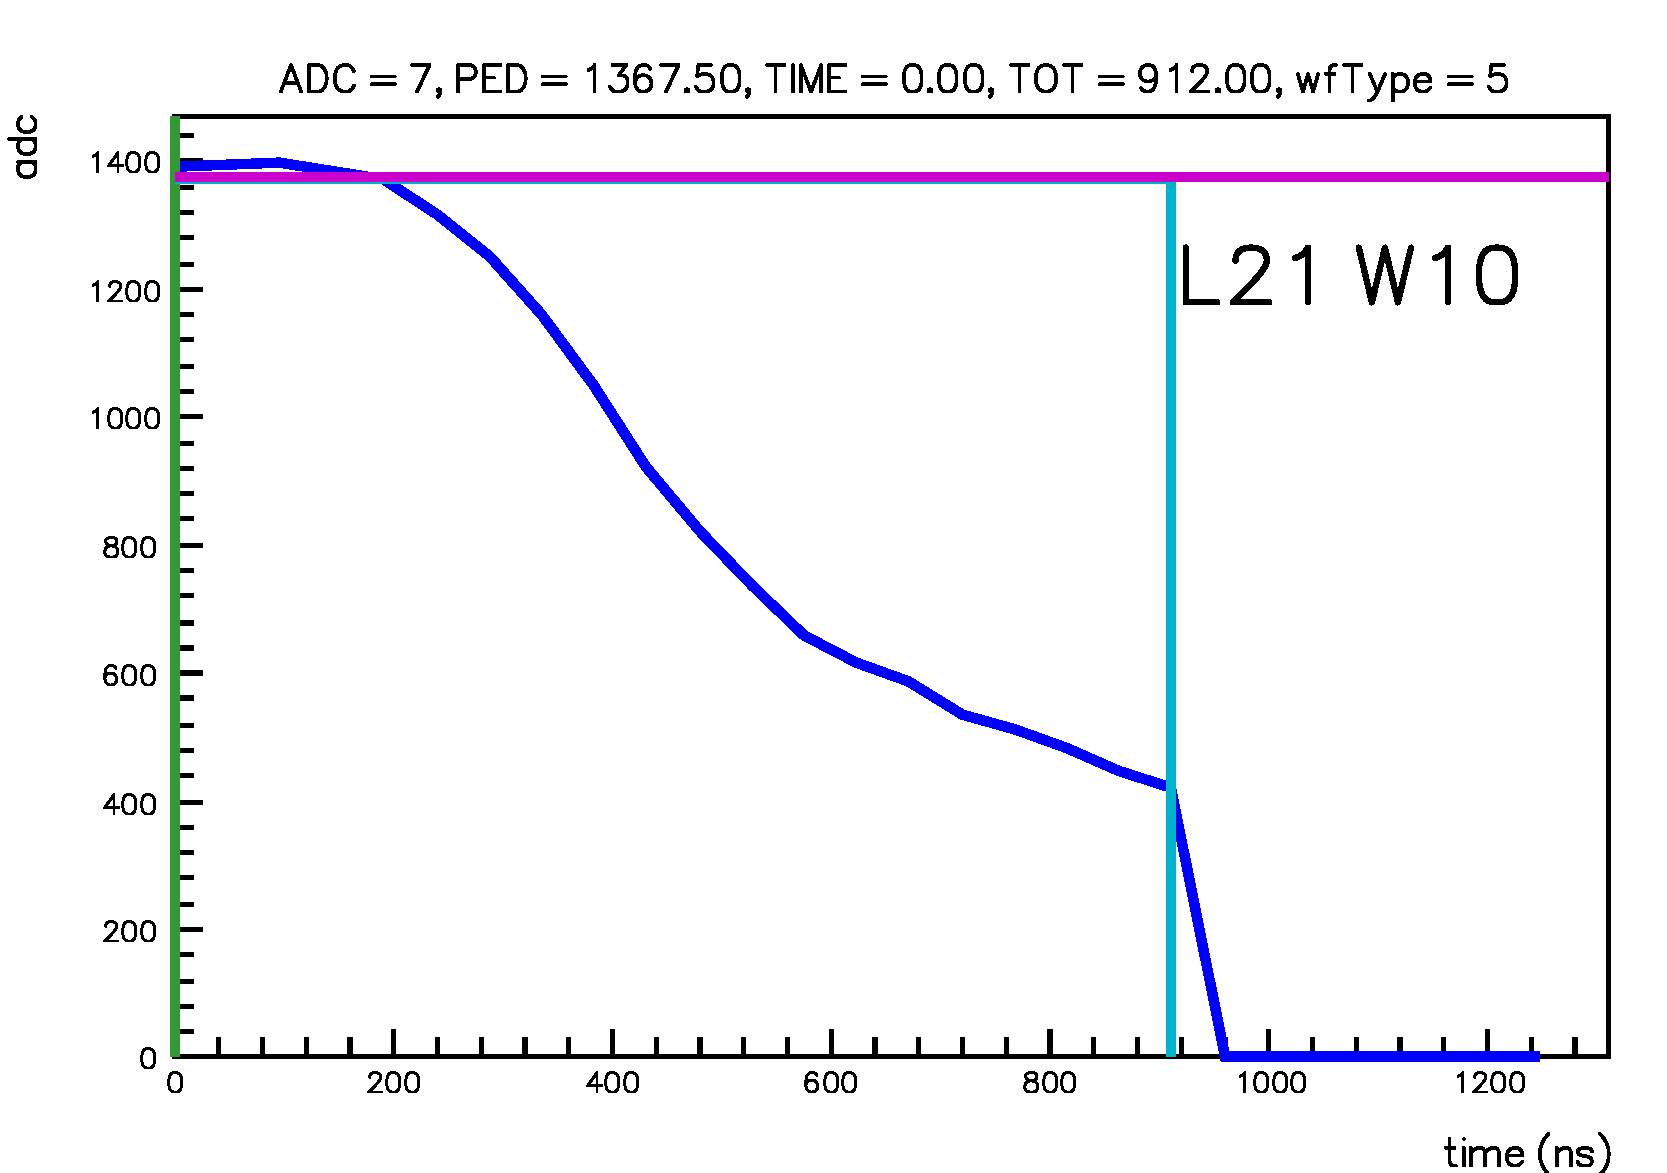
\includegraphics[width=0.24\linewidth]{figures/wf5_decreasing.pdf} &
                    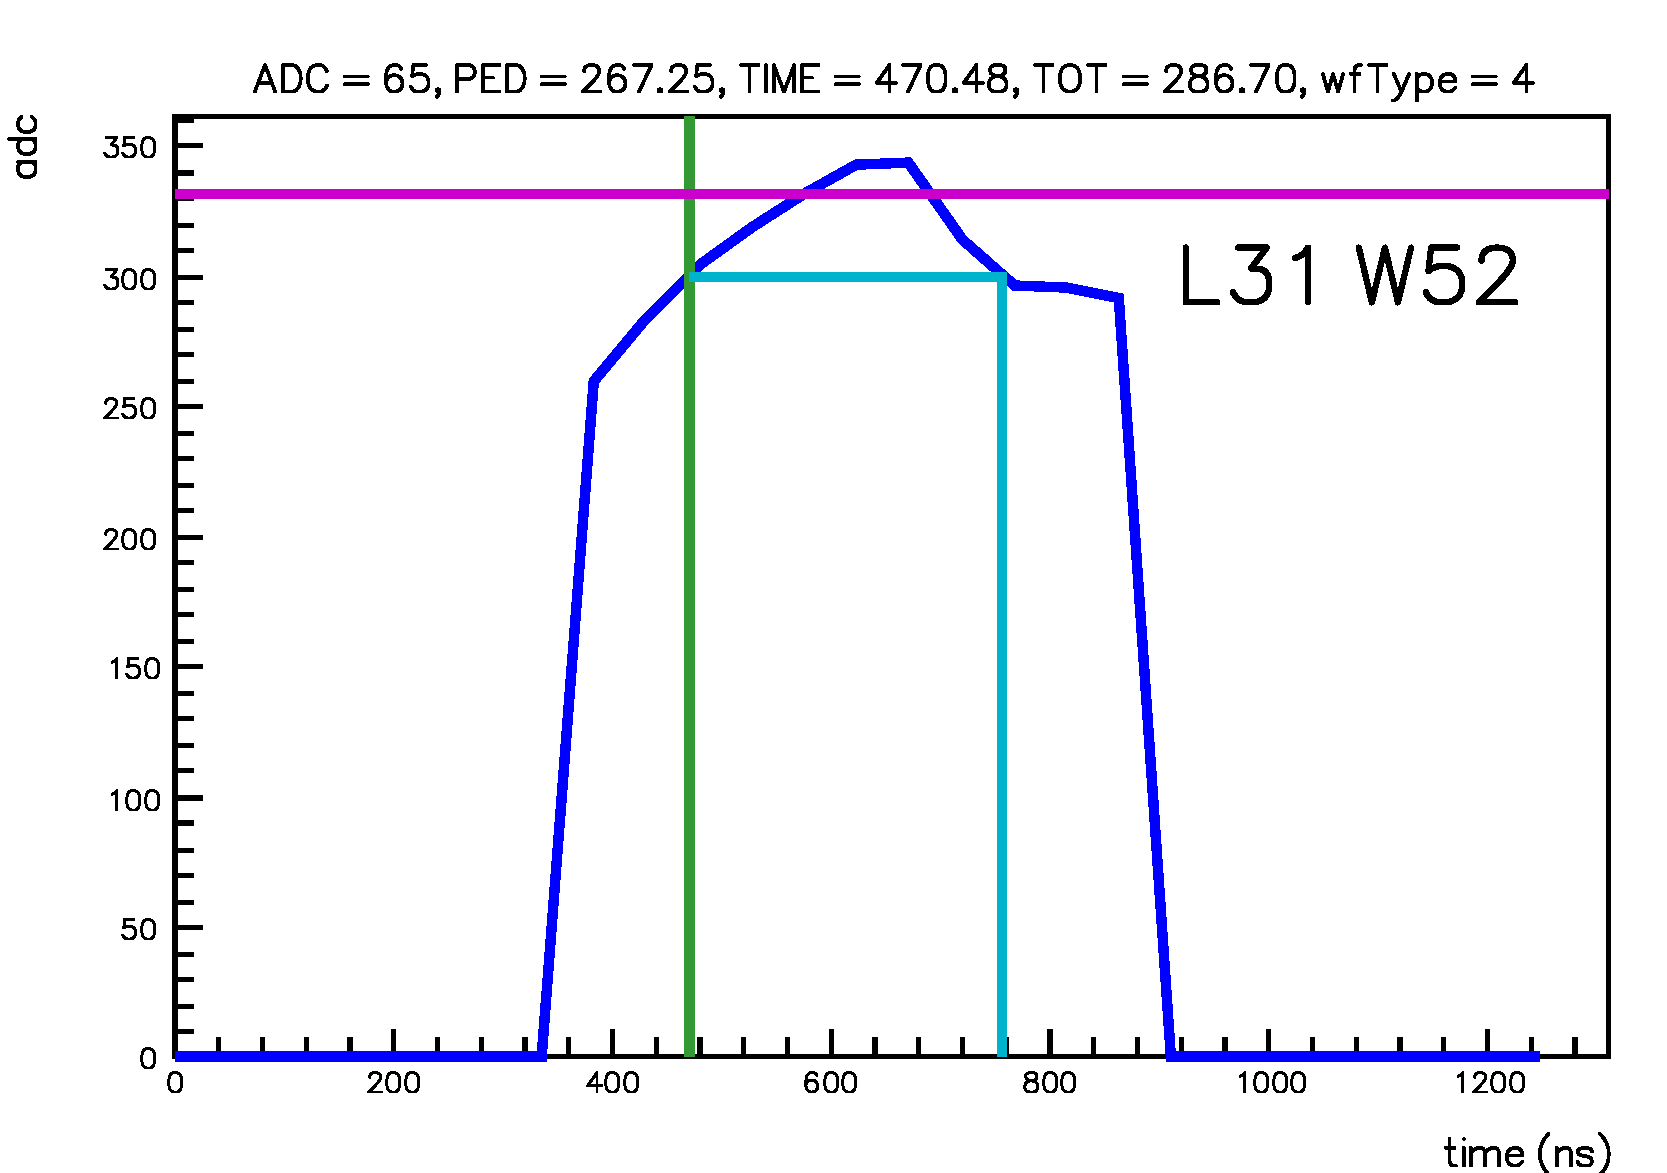
\includegraphics[width=0.24\linewidth]{figures/wf4_bad_tot.pdf} & 
                        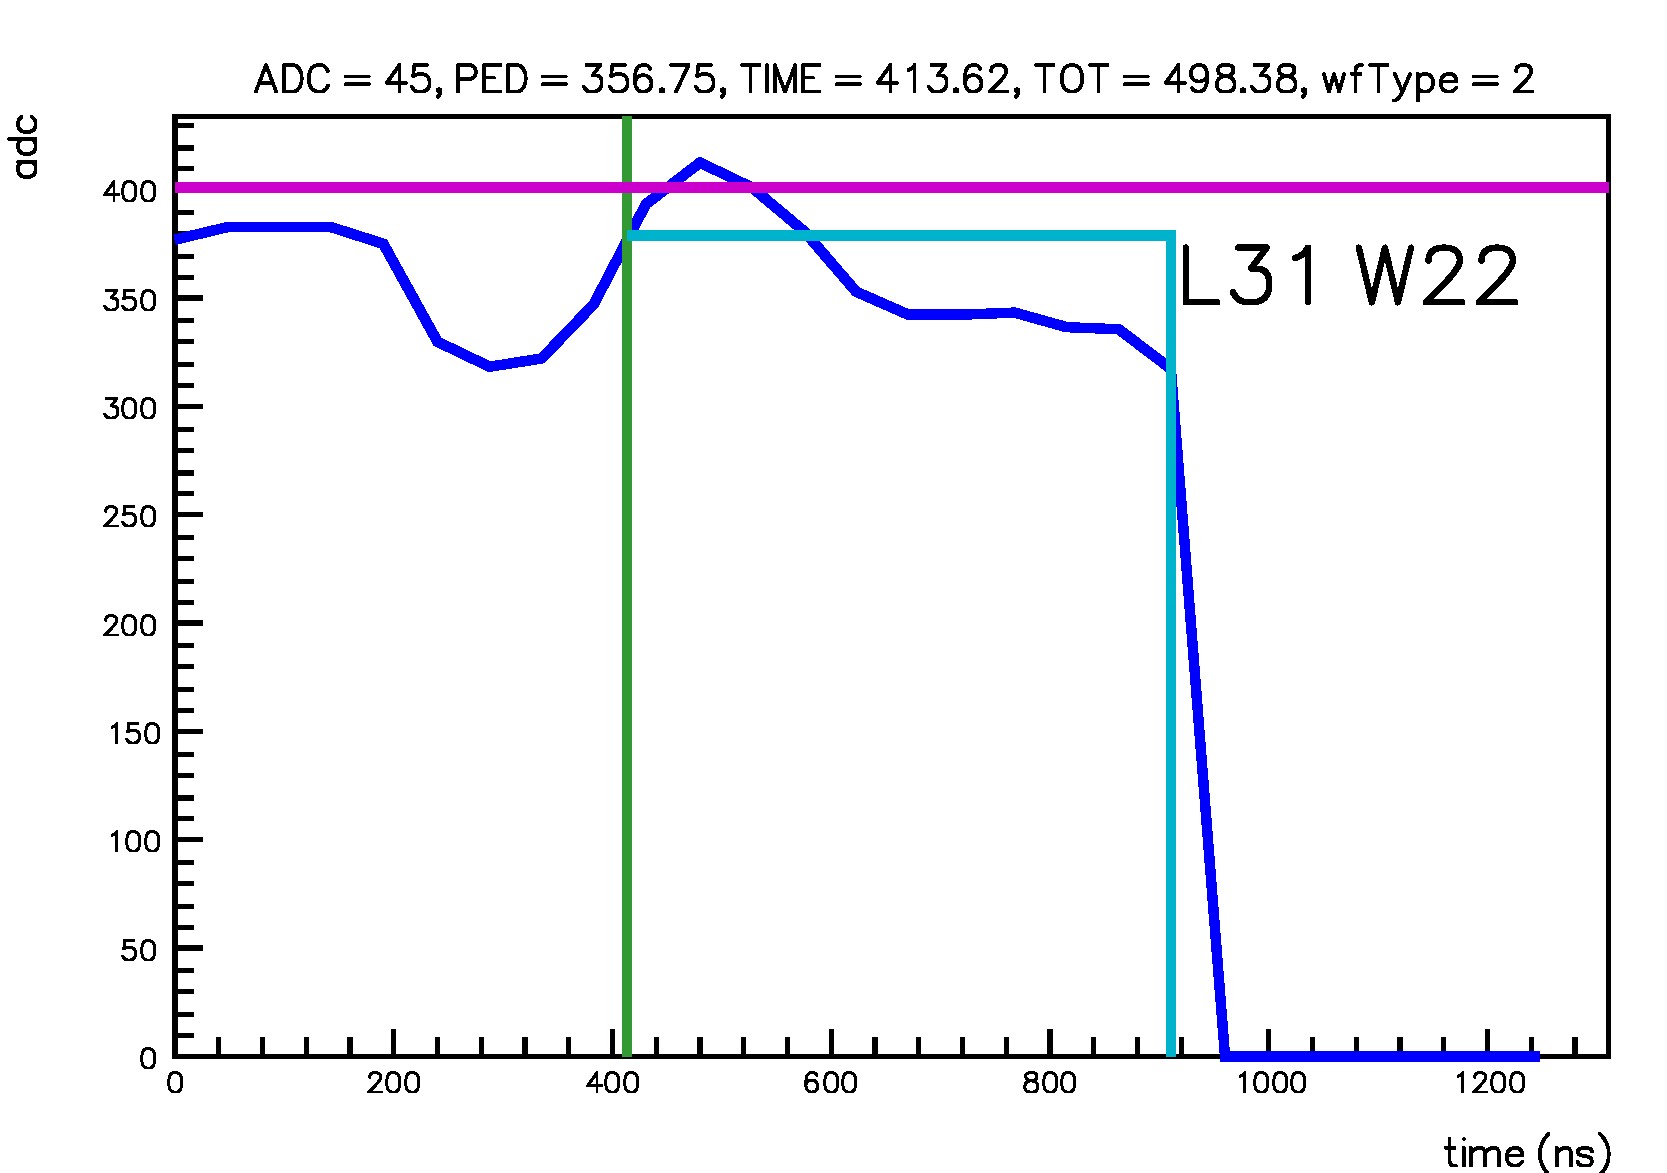
\includegraphics[width=0.24\linewidth]{figures/wf3_pileup.pdf} \\
            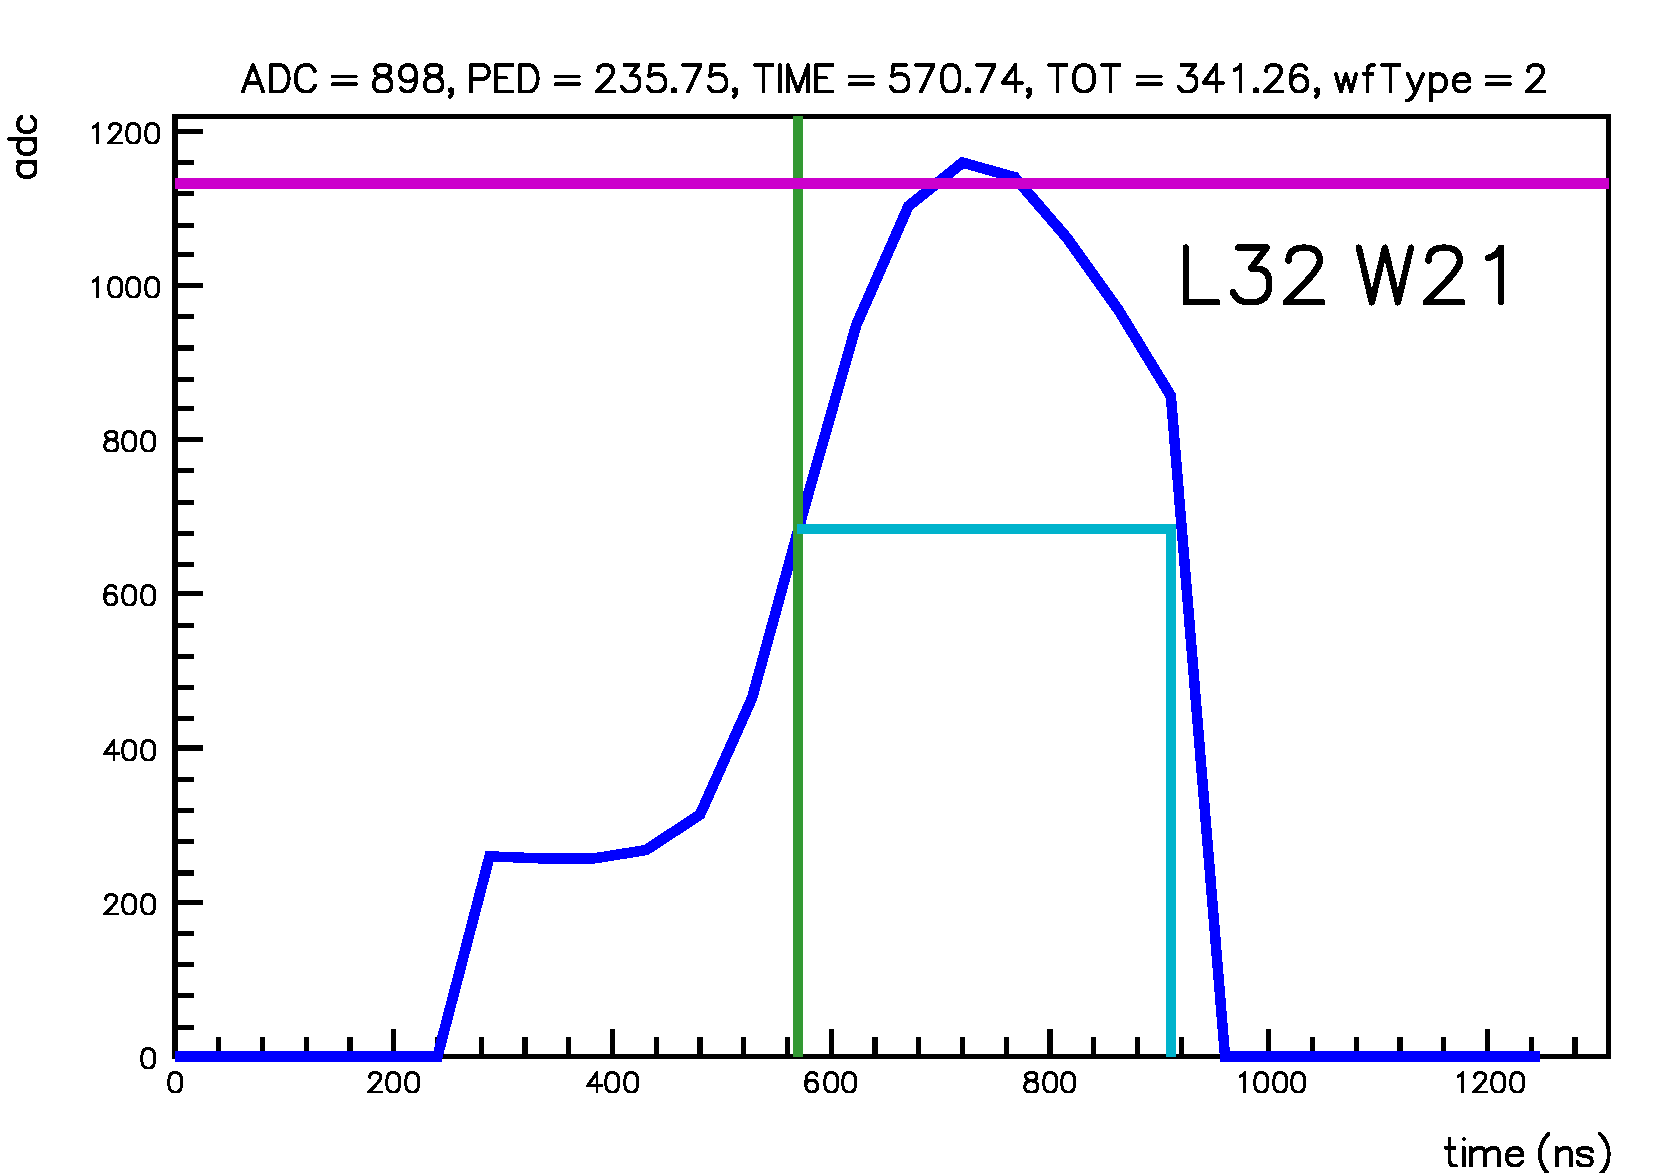
\includegraphics[width=0.24\linewidth]{figures/wf2_bad_trailing_edge.pdf} &
                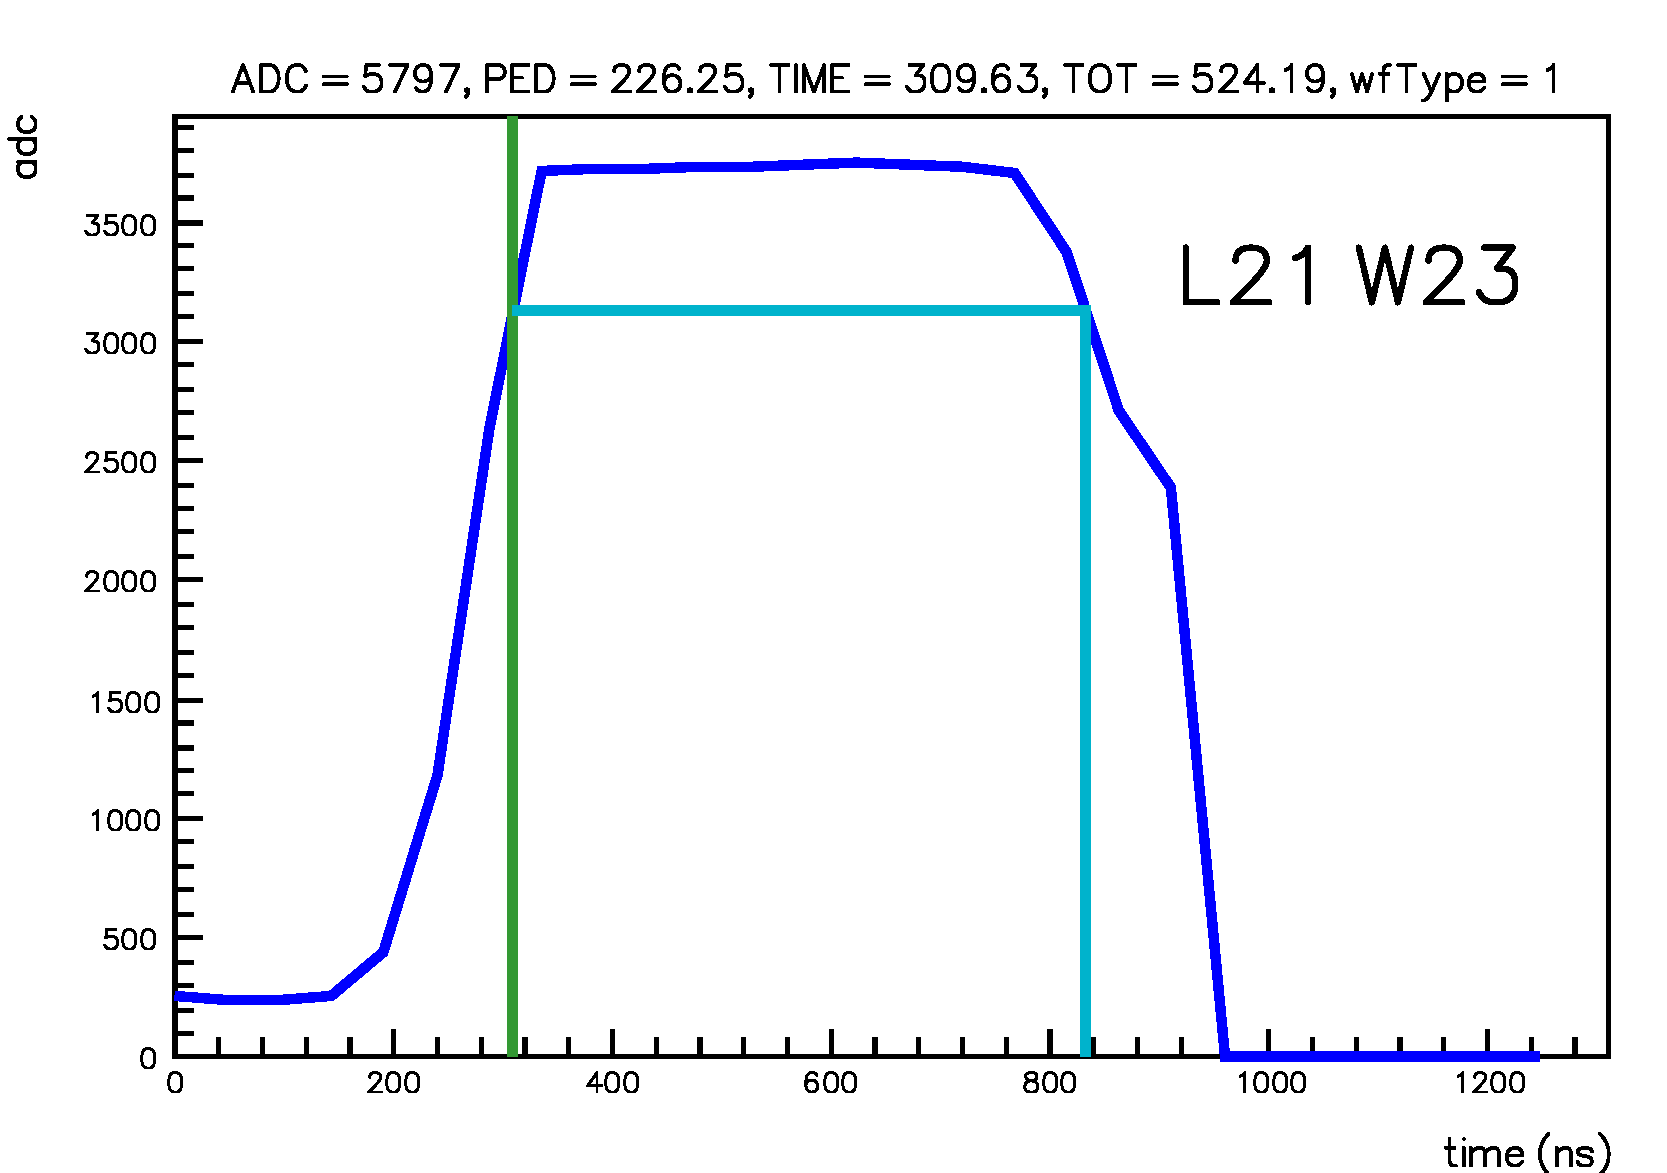
\includegraphics[width=0.24\linewidth]{figures/wf1_saturated.pdf} &
                    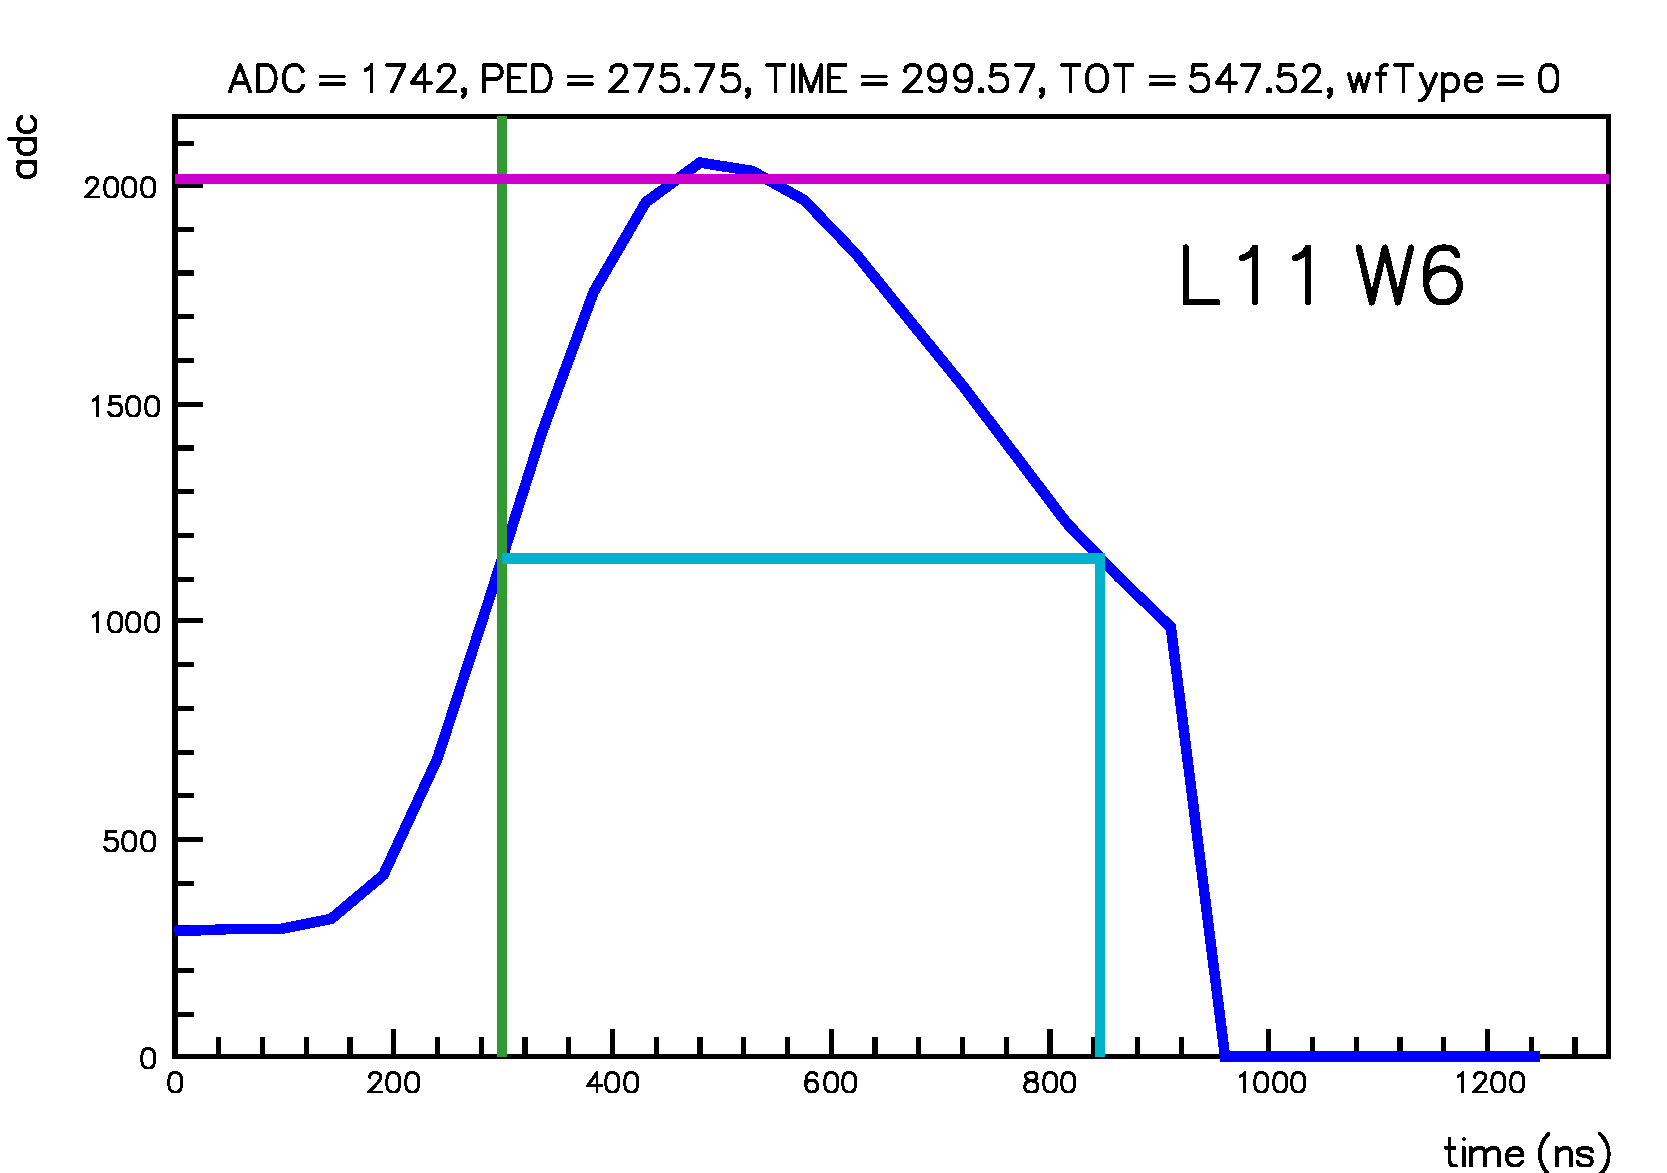
\includegraphics[width=0.24\linewidth]{figures/wf0_normal.pdf} &
        \end{tabular}
    }

    \begin{itemize}
        \item Only signals with a good leading edge time are relevant (wfType $\leq$ 2)
    \end{itemize}
    
\end{frame}

\begin{frame}{Pulse decoding}
    \begin{itemize}
        \item Procedure for extracting the time
            \begin{itemize} \footnotesize
                \item Baseline $\rightarrow$ estimated using the 4 first samples
                \item Amplitude $\rightarrow$ after baseline subtraction, average of 3 samples around the peak
                \item Leading edge time $\rightarrow$ computed at 1/2 amplitude
                \item Time over threshold $\rightarrow$ computed if the signal has a trailing edge at 1/2 amplitude
            \end{itemize}
    \end{itemize}
    
    \vspace{0.3cm}
    \centering
    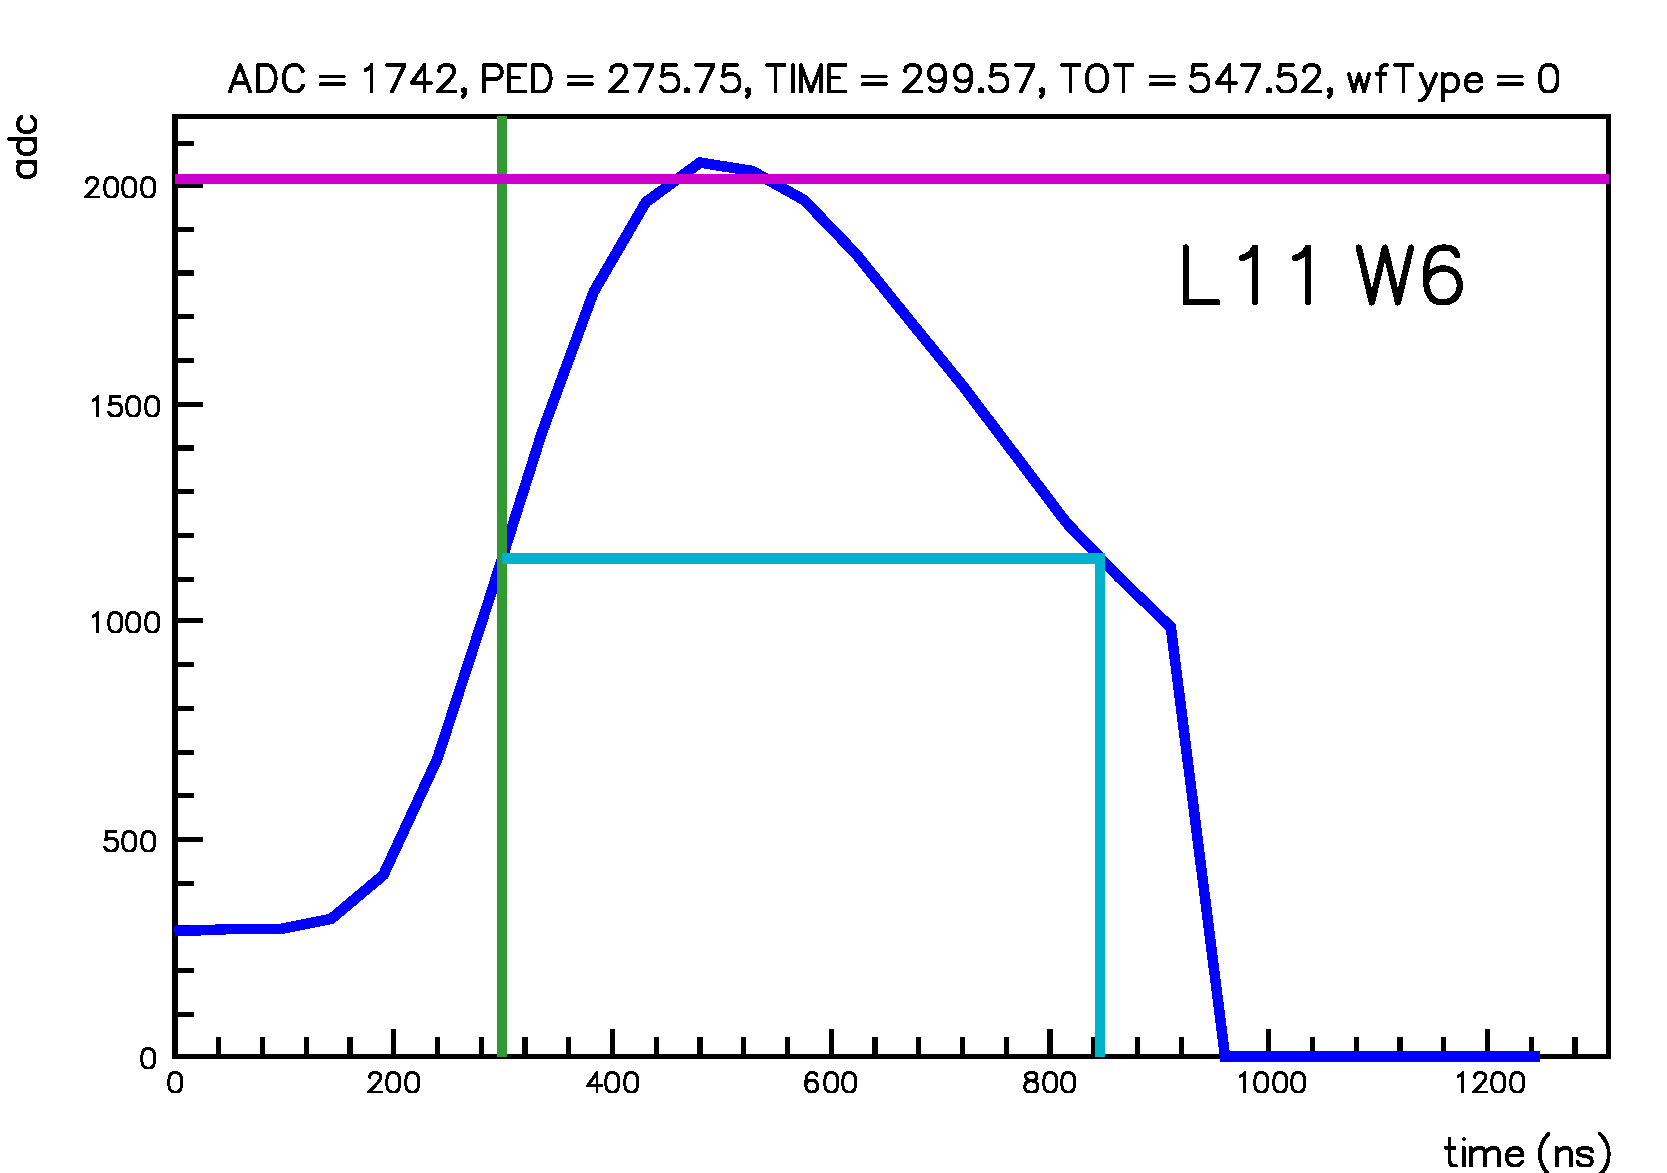
\includegraphics[width=0.6\linewidth]{figures/wf0_normal.pdf} 
    % \includegraphics[width=0.44\linewidth]{figures/build/adc_of_saturated_signals.pdf}

    % \begin{minipage}{0.4\linewidth}
    %     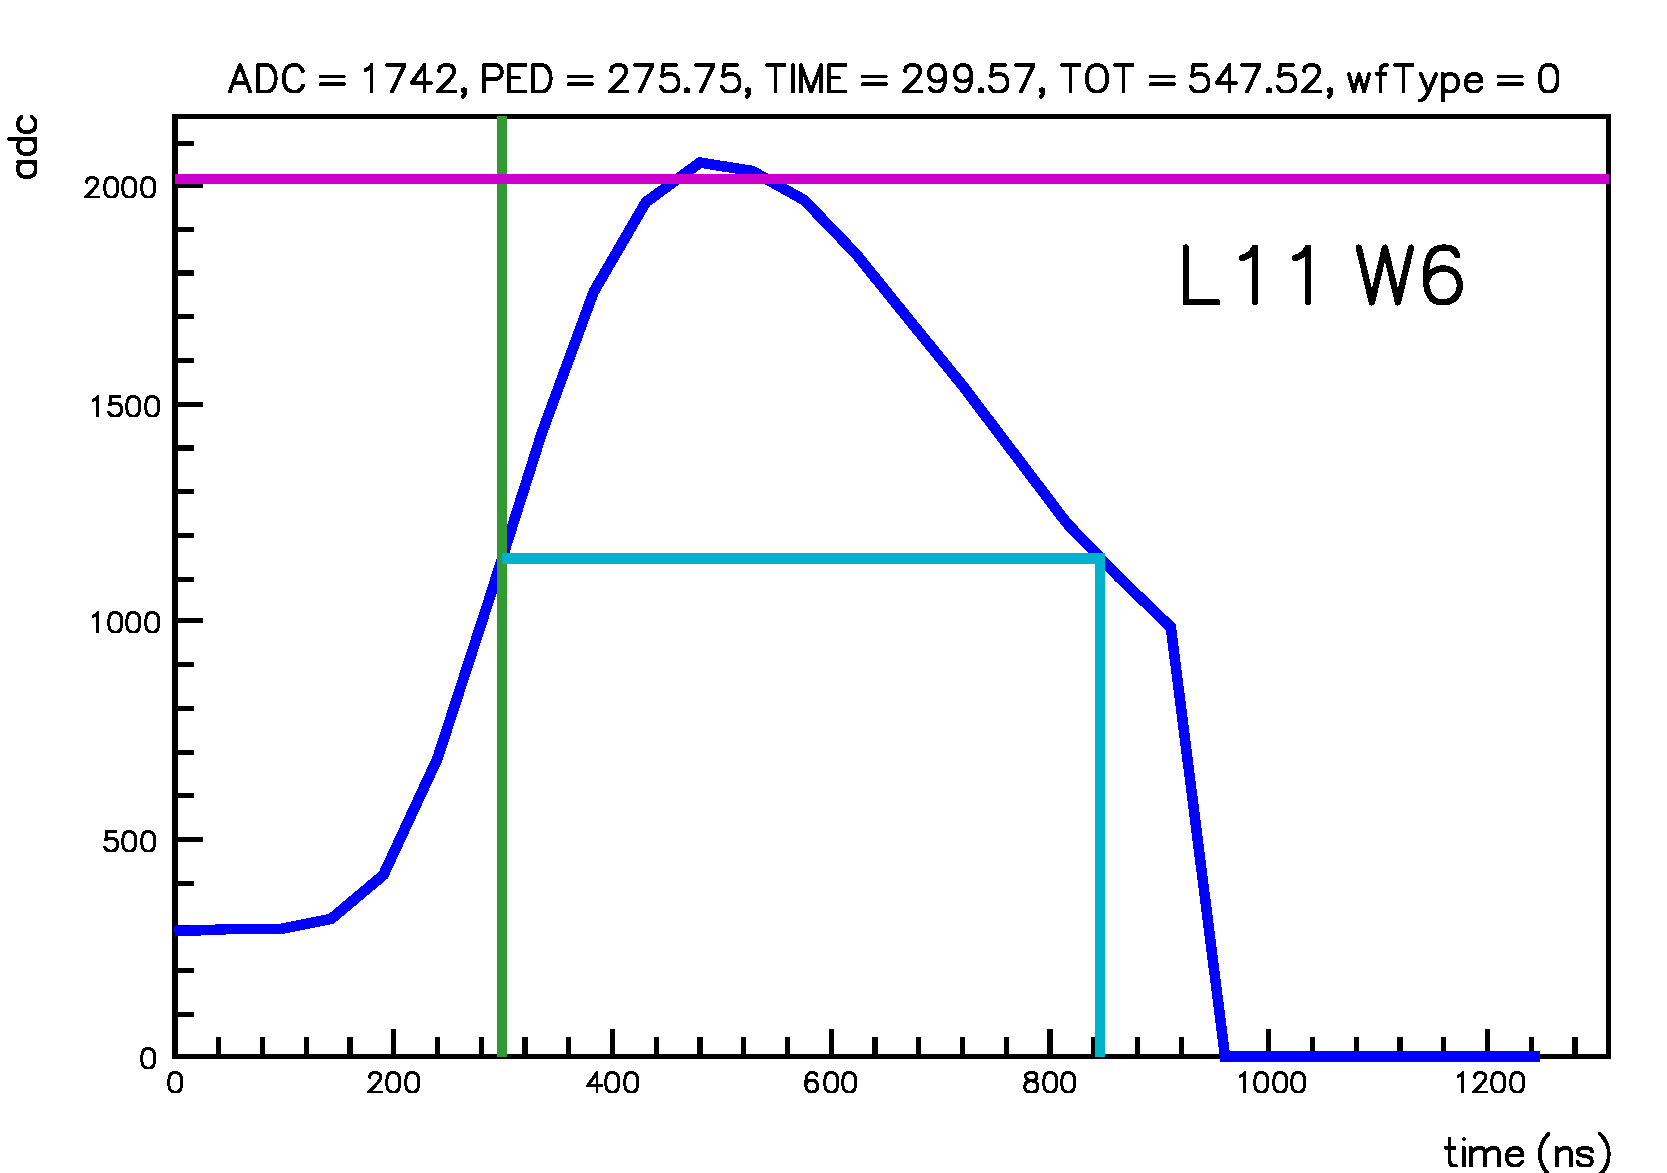
\includegraphics[width=\linewidth]{figures/wf0_normal.pdf} 
    % \end{minipage}
    % \begin{minipage}{0.42\linewidth}
    %     \includegraphics[width=\linewidth]{figures/build/adc_of_saturated_signals.pdf} 
    % \end{minipage}

    
\end{frame}

\begin{frame}{Decoding of saturated signals}

    \begin{minipage}{0.6\linewidth}
        \begin{itemize}
            \item The signals of $\alpha$ particles always saturate
            \item The time extracted at 1/2 saturated ADC is under-estimated
                \begin{itemize}
                    \item It badly impacts the reconstruction
                \end{itemize}
            \item To correct for the amplitude, we use the linear correlation of the maximum slope of a non-saturated signal with its amplitude
            \item With the corrected amplitude, we can recompute the time at 1/2 amplitude
        \end{itemize}

        \centering
        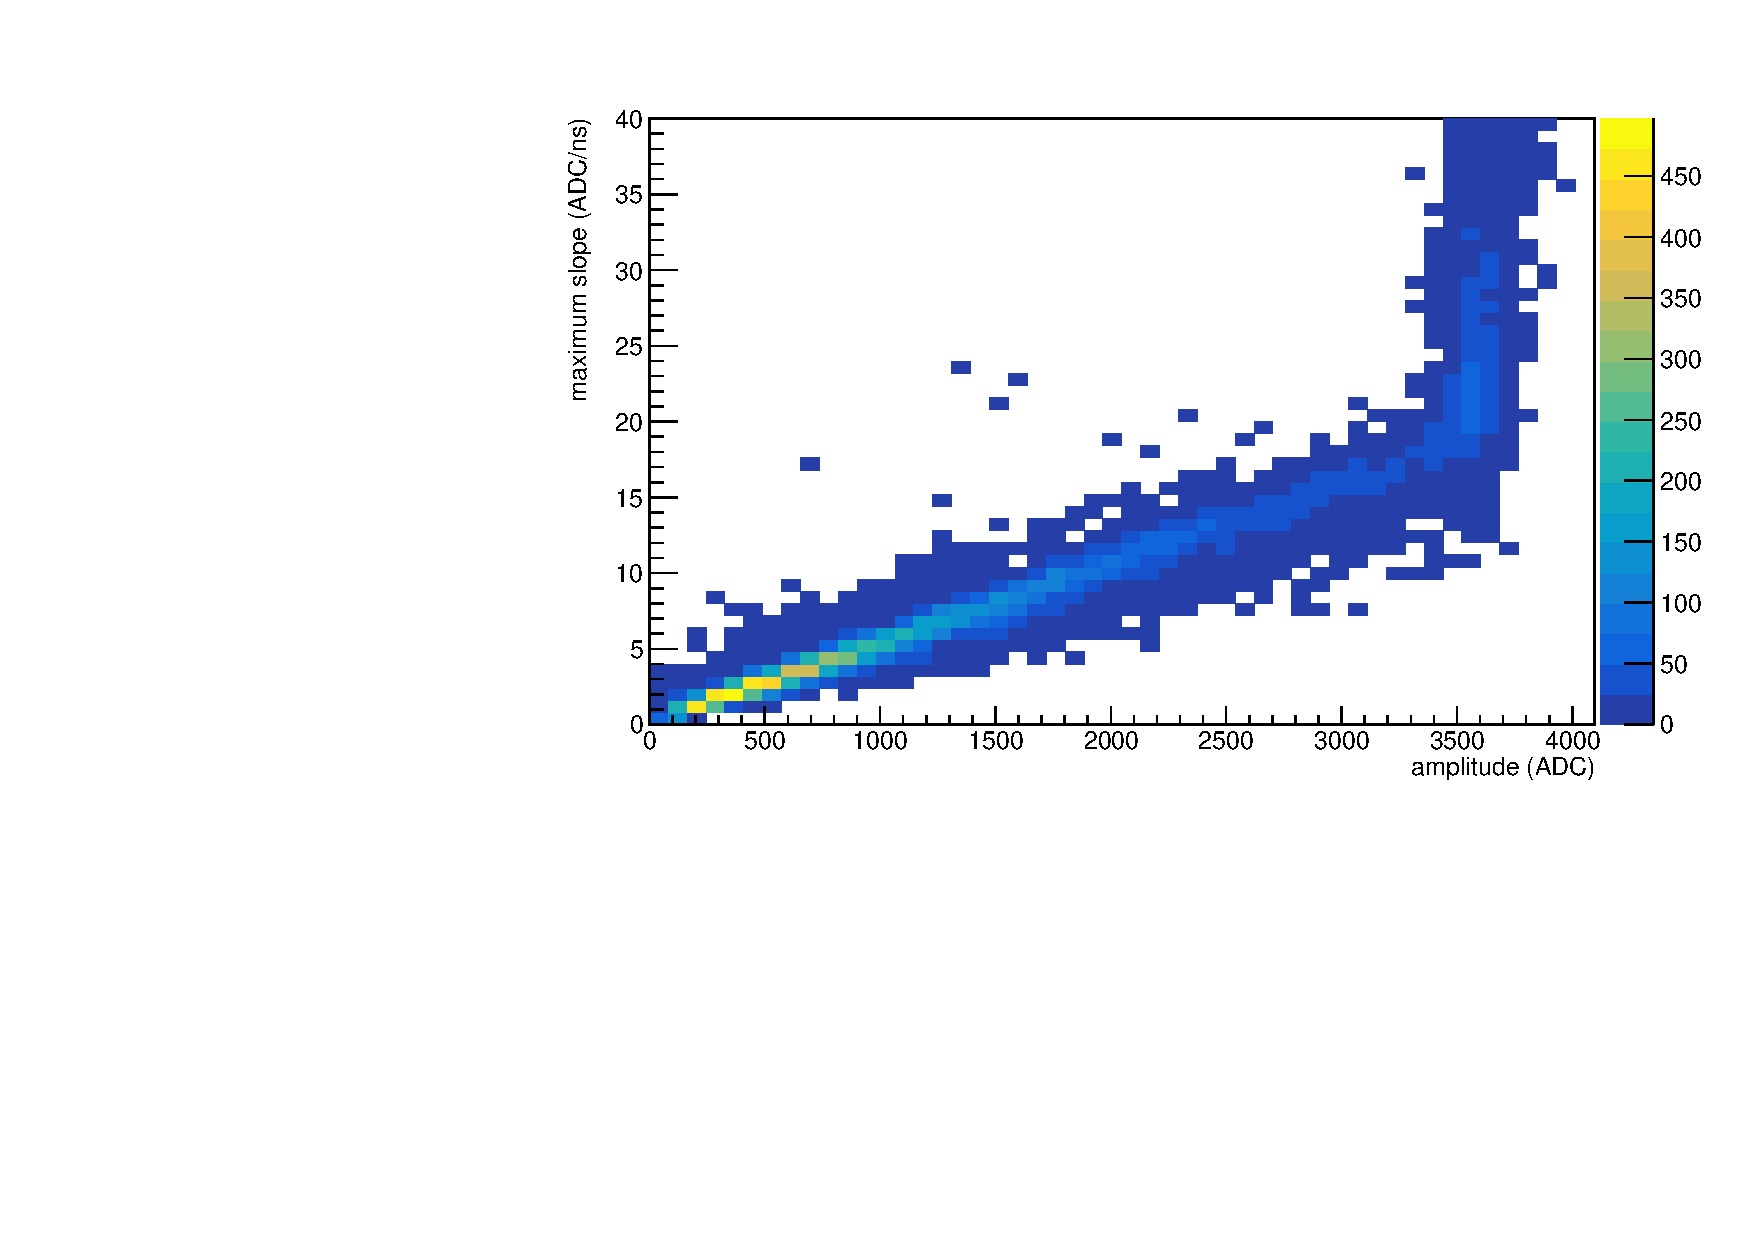
\includegraphics[width=0.7\linewidth]{figures/slope_versus_adc_all_signals.pdf} 
    \end{minipage}
    \begin{minipage}{0.37\linewidth}
        \includegraphics[width=\linewidth]{figures/build/adc_of_saturated_signals.pdf}

        \vspace{0.3cm}

        \includegraphics[width=\linewidth]{figures/build/decoding_saturated_signals_normal.pdf}

        \begin{itemize}
            \item This method has been compared with the one based on the time over threshold
        \end{itemize}
    \end{minipage}    
    
\end{frame}

\begin{frame}[fragile]{Typical hit selection}
    \begin{itemize}
        \item Electron (pid=11, $W^2$ cut for elastics)
        \item Track (AHDC::kftrack)
            \begin{itemize}
                \item nb. hits $\geq$ 7
                \item $\chi^2 < 8$
                \item $\Delta \phi$ cut for elastics
            \end{itemize}
        \item Hit (AHDC::hits)
            \begin{itemize}
                \item The track id should match the one from an existing track
                \item Example of code :
            \end{itemize}
    \end{itemize}

\vspace{0.3cm}
\centering
\begin{minipage}{0.9\linewidth}
\begin{lstlisting}
int trackid = trackBank.getInt("trackid", i);
for (int j = 0; j < hitBank.getRows(); j++) {
    if (hitBank.getInt("trackid", j) == trackid) {
        double residual = hitBank.getDouble("residual", j);
        double time = hitBank.getDouble("time", j);
        int adcRow = hitBank.getShort("id", j) - 1;
        // moving from hit row to adc row !
        int wfType = adcBank.getShort("wfType", adcRow);
        double leadingEdgeTime = adcBank.getShort("leadingEdgeTime", adcRow);
        // etc.
    }
}
\end{lstlisting} 
\end{minipage}

\end{frame}



\end{document}


